%----------- slide --------------------------------------------------%
\begin{frame}
\frametitle{{\airs} and {\cris} Sampling}

\begin{itemize}

  \item we want to compare {\airs} and {\cris} obs coverage.  Both
    are in sun-synchronous polar orbits

  \item the {\cris} orbital period is 101.5 minutes $\pm 0.2$
    seconds, giving 227 orbits every 16 days

  \item the {\airs} orbital period 98.8 minutes, giving 233 orbits
    every 16 days

  \item 227 and 233 are both prime; there are no common factors and
    so no repeating subpatterns

  \item the scan patterns and in particular the secant of zenith
    angles are relatively close, as shown in a subsequent slide

\end{itemize}
\end{frame}
%----------- slide --------------------------------------------------%
\begin{frame}
\frametitle{one-day track map}
\begin{center}
  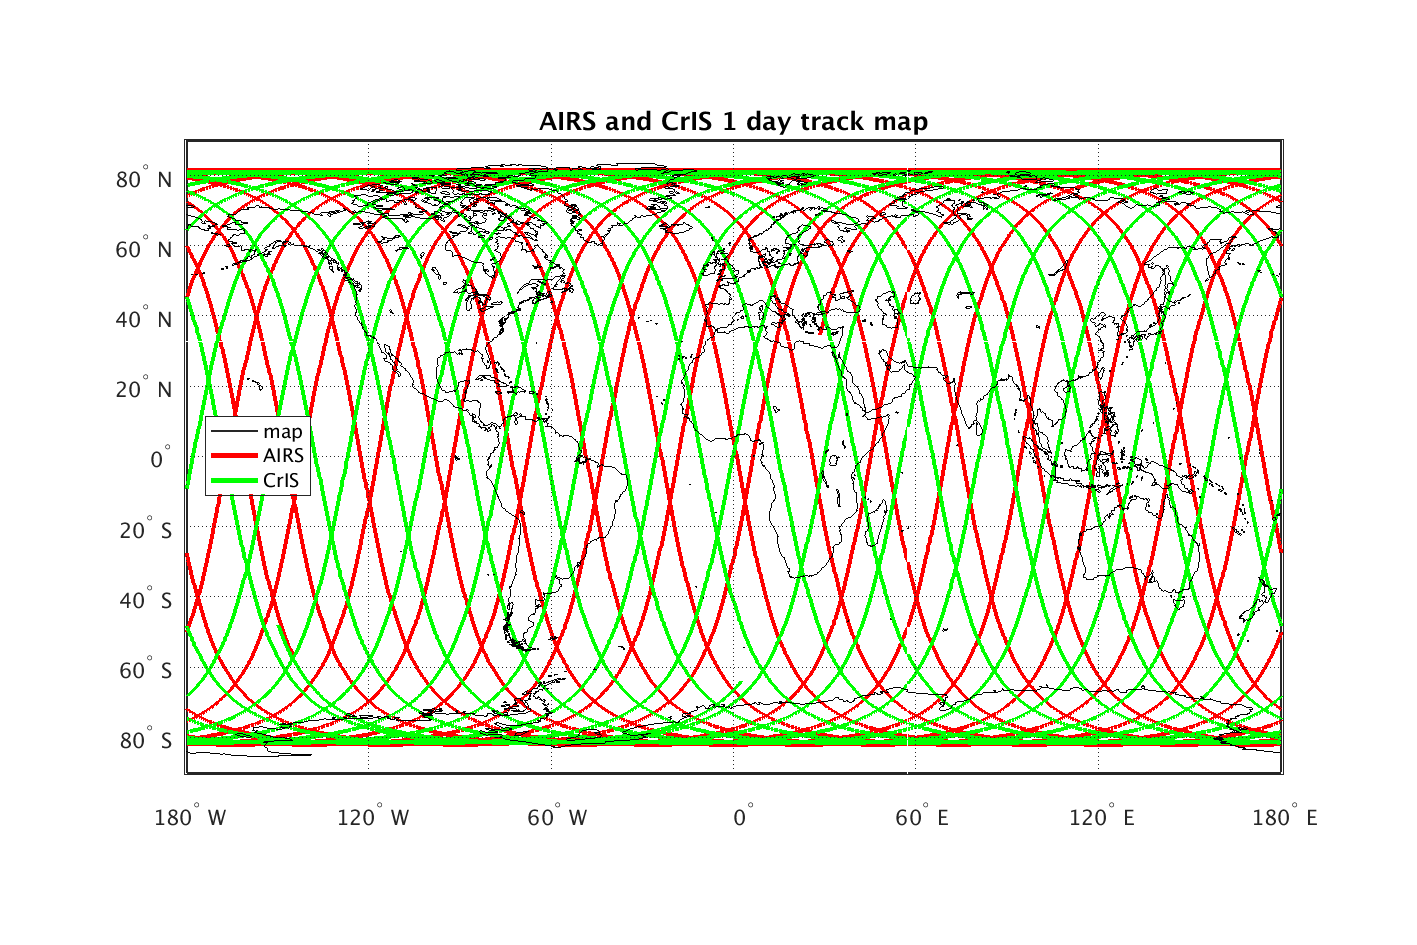
\includegraphics[scale=0.5]{figures/subpt_1_day_all.png}
\end{center}
\end{frame} % source plot_subpt.m
%----------- slide --------------------------------------------------%
\begin{frame}
\frametitle{16 day track maps}
\begin{center}
  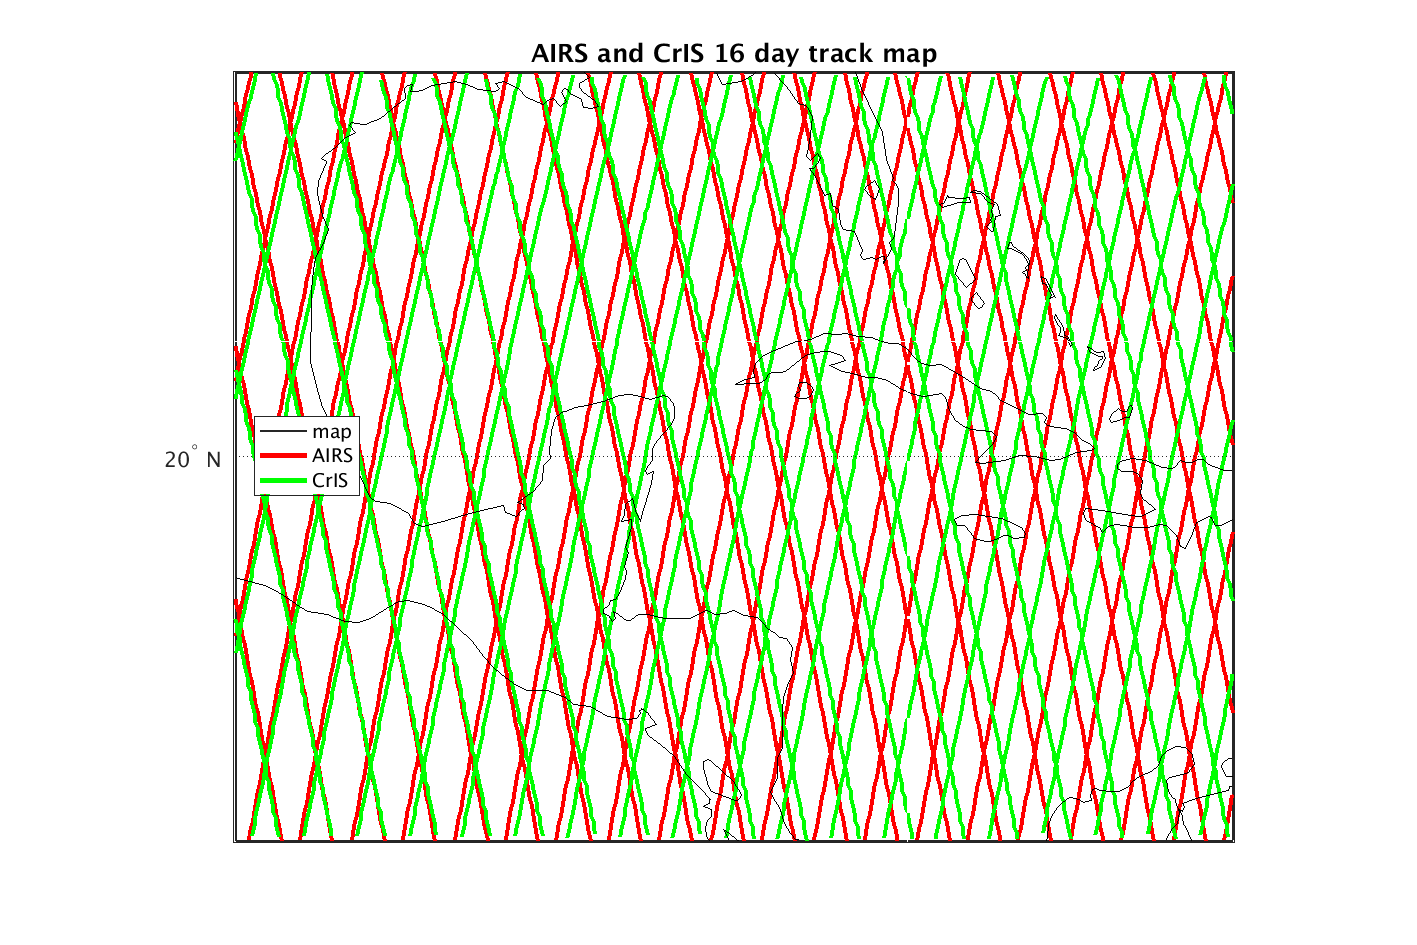
\includegraphics[scale=0.5]{figures/subpt_16_day_zoom.png}
\end{center}
\end{frame} % source plot_subpt.m
%----------- slide --------------------------------------------------%
\begin{frame}
\frametitle{{\airs} and {\cris} secant of zenith angles}

\begin{center}
  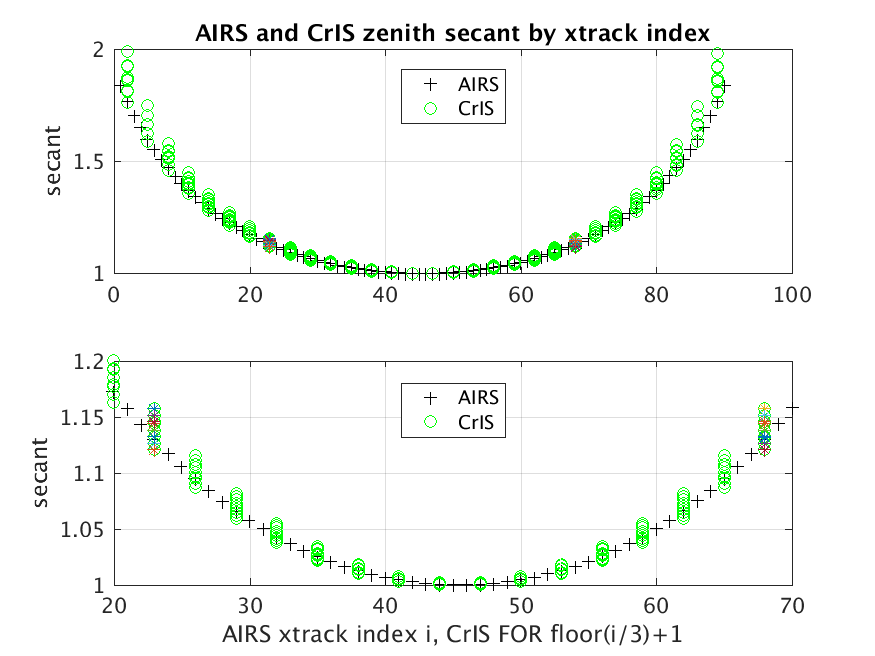
\includegraphics[scale=0.7]{figures/AIRS_CrIS_secant_by_xtrack.png}
\end{center}
\end{frame} % source plot_tbin.m
%----------- slide --------------------------------------------------%
\begin{frame}
\frametitle{{\airs} to {\cris} statistical correction}
\begin{itemize}

  \item We can further reduce the residuals with a simple linear or
    quadratic correction, applied independently to each channel.

  \item We use a set of 7377 radiances calculated from all-sky {\airs}
    profiles spanning several consecutive days as the dependent set.

  \item Let $\Ttc_i$ be true {\cris} and $\Tac_i$ {\airs} {\cris}
    brightness temperatures for {\cris} channel $i$, from the
    dependent set.

  \item For the bias test we subtract the mean residual from the
    dependent set.  For the linear test we find $a_i$ and $b_i$ to
    minimize $||a_i\,\Tac_i + b_i - \Ttc_i||_2$, and for the
    quadratic test $c_i$, $a_i$ and $b_i$ to minimize
    $||c_i\,(\Tac_i)^2 + a_i\,\Tac_i + b_i - \Ttc_i||_2$.

  \item The $a$ weights are very close to 1, the $b$ weight to the
    bias, and the $c$ weights to zero.  The linear correction worked
    best.

  \item The resulting correction is applied to the independent set,
    the 49 fitting profiles, for comparison with true {\cris}.  This
    gives a stricter test than splitting the more correlated 7377
    profile set into dependent and independent subsets.

\end{itemize}
\end{frame}
%----------- slide --------------------------------------------------%
\begin{frame}
\frametitle{{\airs} to {\cris} statistical correction}
\begin{columns}[t]
\begin{column}{0.5\textwidth}
  \begin{centering}
  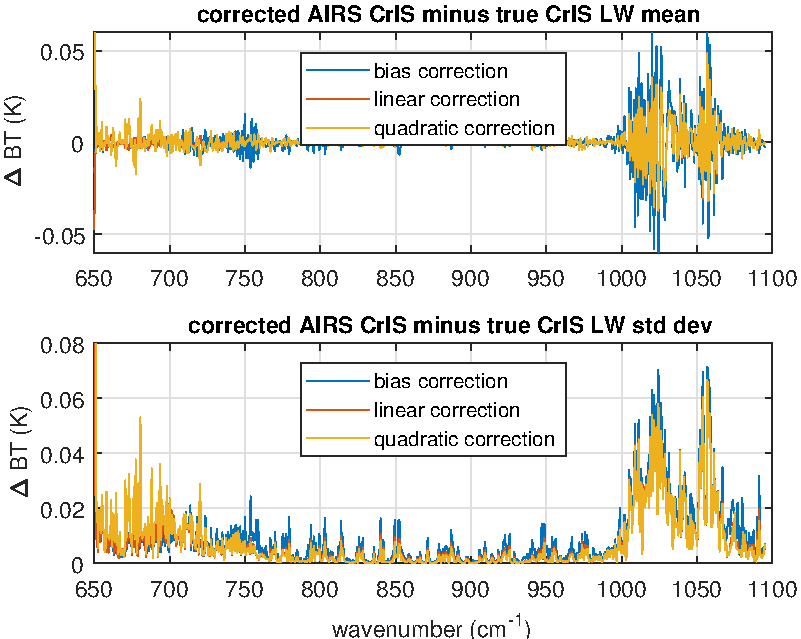
\includegraphics[width=\textwidth]{figures/a2cris_regr_LW.pdf}
  \end{centering}\vspace{3mm}
  Mean and standard deviation of LW corrected apodized residuals.

\end{column}
\begin{column}{0.5\textwidth}
  \begin{centering}
  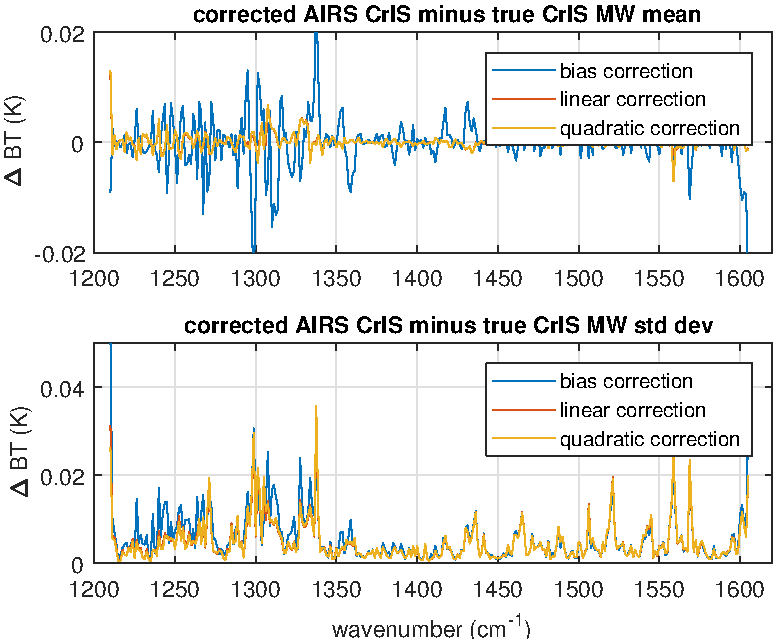
\includegraphics[width=\textwidth]{figures/a2cris_regr_MW.pdf}
  \end{centering}\vspace{3mm}
  Mean and standard deviation of MW corrected apodized residuals.
 
\end{column}
\end{columns}
\end{frame}
%----------- slide --------------------------------------------------%
\begin{frame}
\frametitle{{\airs} to {\cris} statistical correction}
\begin{columns}[t]
\begin{column}{0.5\textwidth}  
  \begin{centering}
  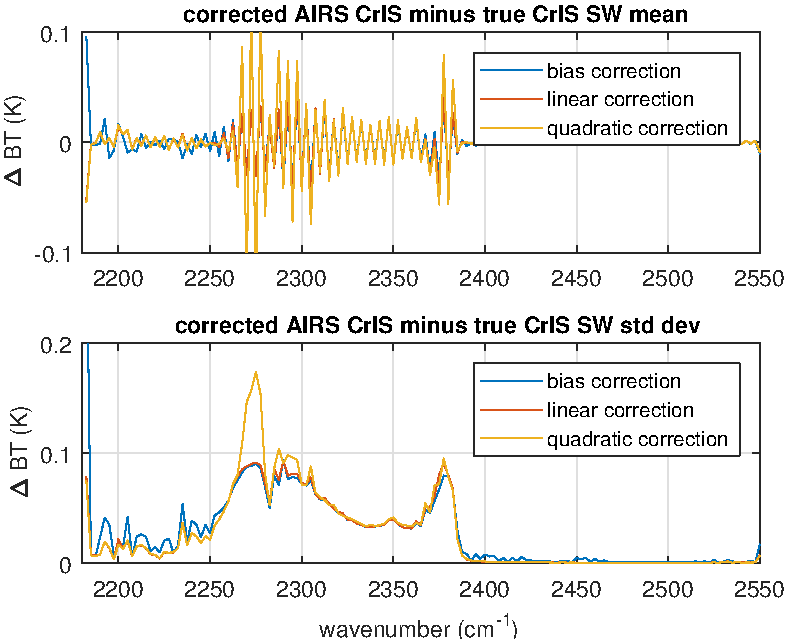
\includegraphics[width=\textwidth]{figures/a2cris_regr_SW.pdf}
  \end{centering}\vspace{3mm}
  Mean and standard deviation of SW corrected apodized residuals.

\end{column}
\begin{column}{0.5\textwidth}
  \begin{centering}
  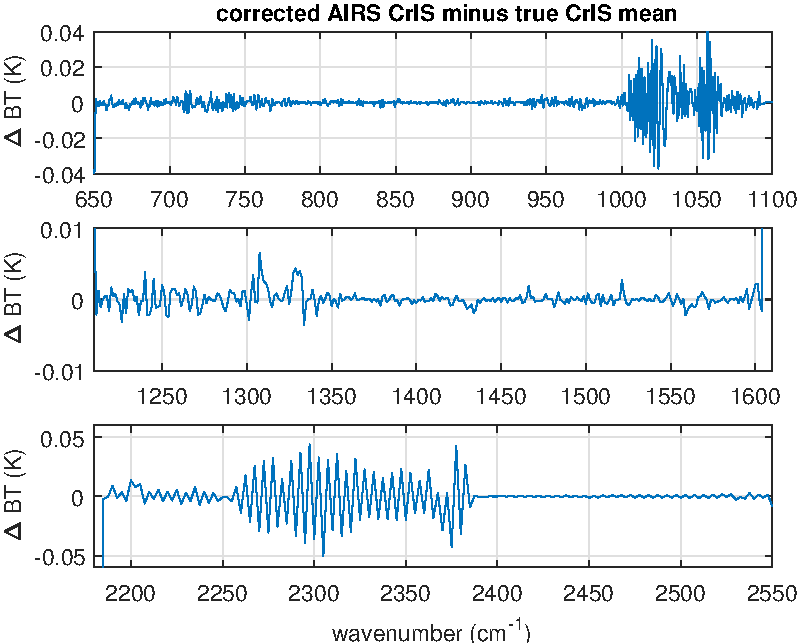
\includegraphics[width=\textwidth]{figures/ap_decon_corr.pdf}
  \end{centering}\vspace{3mm}
  Mean corrected apodized residuals for all three bands, showing
  the linear corrected apodized residuals in greater detail.
\end{column}
\end{columns}
\end{frame}
%----------- slide --------------------------------------------------%
\begin{frame}
\frametitle{Conclusions}
\begin{itemize}

  \item We have done a preliminary analysis of the MN Plateau 22
    CH$_4$, CO$_2$, and CO gas cell tests, and compared these with
    calculated reference truth.  Overall, the results look quite
    good.

  \item The HTBB drift seen in many of the test legs is significant
    but managable with our approach to regression fitting.   The effect
    of the drifts could be reduced with more careful subsetting, if
    needed.

  \item Metrology laser relative residuals are in reasonable
    agreement, and can be reduced further with focal plane
    adjustments.  Metrology laser absolute residuals could be
    reduced with a more judicious choice of neon wavelengh, or 
    possibly by simply using the eng neon value.

\end{itemize}
\end{frame}
